\documentclass[oneside,a4paper,14pt]{extarticle}
\usepackage[T1,T2A,TU]{fontenc}
\usepackage[a4paper,letterpaper,top=20mm,bottom=20mm,left=20mm,right=10mm]{geometry}
\usepackage[russian]{babel}
\usepackage{textcomp}
\usepackage{indentfirst}
\usepackage{graphicx}
\usepackage{mwe}
\usepackage{wrapfig}
\usepackage{caption}
\usepackage{amsmath}
\usepackage{amsfonts}
\usepackage{amsthm}
\usepackage{amssymb}
\usepackage[all]{xy}
\usepackage[breaklinks]{hyperref}
\usepackage{titlesec}
\usepackage{verbatim, fancyvrb}

\titleformat{\section} % Настройка формата заголовков секций
{\normalsize\bfseries} % Устанавливает размер шрифта на нормальный и делает его жирным
{\thesection} % Указывает, что номер секции будет отображаться перед заголовком
{1em} % Устанавливает расстояние между номером секции и заголовком в 1em
{} % Дополнительные параметры.

\titleformat{\subsection} % Настройка формата заголовков подсекций
{\normalsize\bfseries} % Устанавливает размер шрифта на нормальный и делает его жирным
{\thesubsection} % Указывает, что номер подсекции будет отображаться перед заголовком
{1em} % Устанавливает расстояние между номером подсекции и заголовком в 1em
{} % Дополнительные параметры.

\titleformat{\subsubsection} % Настройка формата заголовков подподсекций
{\normalsize\bfseries} % Устанавливает размер шрифта на нормальный и делает его жирным
{\thesubsection} % Указывает, что номер подподсекции будет отображаться перед заголовком
{1em} % Устанавливает расстояние между номером подподсекции и заголовком в 1em
{} % Дополнительные параметры.

\renewcommand\baselinestretch{1.45}\normalsize %межстр интервал
\setlength{\parindent}{1.25cm} %длина отступа нового абзаца

\begin{document}
\newpage
\thispagestyle{empty}
\begin{center}
	МИНИСТЕРСТВО НАУКИ И ВЫСШЕГО ОБРАЗОВАНИЯ\\
	РОССИЙСКОЙ ФЕДЕРАЦИИ
	ФЕДЕРАЛЬНОЕ ГОСУДАРСТВЕННОЕ БЮДЖЕТНОЕ\\
	ОБРАЗОВАТЕЛЬНОЕ
	УЧРЕЖДЕНИЕ ВЫСШЕГО ОБРАЗОВАНИЯ\\
	«ВЯТСКИЙ ГОСУДАРСТВЕННЫЙ УНИВЕРСИТЕТ»\\
	Институт математики и информационных систем\\
	Факультет автоматики и вычислительной техники\\
	Кафедра электронных вычислительных машин
\end{center}
\vspace{20mm}

\begin{center}
	Отчёт по лабораторной работе №5\\
	по дисциплине\\
	<<Информатика>>\\
	<<Представление вещественных чисел в формате с плавающей точкой.>>\\
\end{center}
\vspace{40mm}
\noindent
\begin{tabular}{ll}
	Разработал студент гр. ИВТб-1301-05-00 & \rule[-1mm]{30mm}{0.10mm}\,/Черкасов А. А./ \\
	                                       & \hspace{8mm}\footnotesize(подпись)          \\

	Проверил доцент кафедры ЭВМ            & \rule[-1mm]{30mm}{0.10mm}\,/Коржавина А.С./ \\
	                                       & \hspace{8mm}\footnotesize(подпись)          \\
\end{tabular}

\vfill
\begin{center}
	Киров\\
	2024
\end{center}

\newpage\thispagestyle{plain}
\section*{Цель работы}
Цель работы: закрепить на практике знания форматах представления числовой
информации. Написать программы, решающие описанные ниже задачи. Программы должны
работать без ошибок на любых наборах входных данных.

\section*{Задания}
\begin{enumerate}
	\item Представить число в формате с плавающей точкой в n-разрядной сетке.
	      Формат аналогичен IEEE 754. \\
	      \textbf{Формат Ввода.} \\
	      В одной строке вещественное число в десятичной системе счисления, разрядность сетки, число разрядов мантиссы. \\
	      \textbf{Формат Вывода.} \\
	      Строка, отображающая введенное число в формате с плавающей точкой.
	      $$
		      \begin{tabular}{ll}
			      \textbf{Ввод} & \textbf{Вывод}   \\
			      \hline
			      -1.25 16 10   & 1011110100000000 \\
			      \hline
		      \end{tabular}
	      $$
	\item Представить число в формате с плавающей точкой в n-разрядной сетке.
	      Нормализация мантиссы дробная, формат с порядком, последовательность
	      отображения --- знак, мантисса, порядок. \\
	      \textbf{Формат Ввода.} \\
	      В одной строке вещественное число в десятичной системе счисления, разрядность сетки, число разрядов мантиссы. \\
	      \textbf{Формат Вывода.} \\
	      Строка, отображающая введенное число в формате с плавающей точкой.
	      $$
		      \begin{tabular}{ll}
			      \textbf{Ввод} & \textbf{Вывод}   \\
			      \hline
			      -1.25 16 10   & 1101000000000001 \\
			      \hline
		      \end{tabular}
	      $$

	\item Представить число в формате с плавающей точкой в n-разрядной сетке. Нормализация мантиссы дробная, формат с характеристикой, последовательность отображения – знак, мантисса, характеристика. \\
	      \textbf{Формат Ввода.} \\
	      В одной строке вещественное число в десятичной системе счисления, разрядность сетки, число разрядов мантиссы. \\
	      \textbf{Формат Вывода.} \\
	      Строка, отображающая введенное число в формате с плавающей точкой.
	      $$
		      \begin{tabular}{ll}
			      \textbf{Ввод} & \textbf{Вывод}   \\
			      \hline
			      -1.25 16 10   & 1101000000010001 \\
			      \hline
		      \end{tabular}
	      $$
\end{enumerate}
\newpage

\section*{Решение}
\noindent Схема алгоритма представлена на Рисунках 1.1, 1.2 и 1.3. \\
\noindent Код программы приведён в Приложении A1.\\
\begin{figure}[h!]
	\centering
    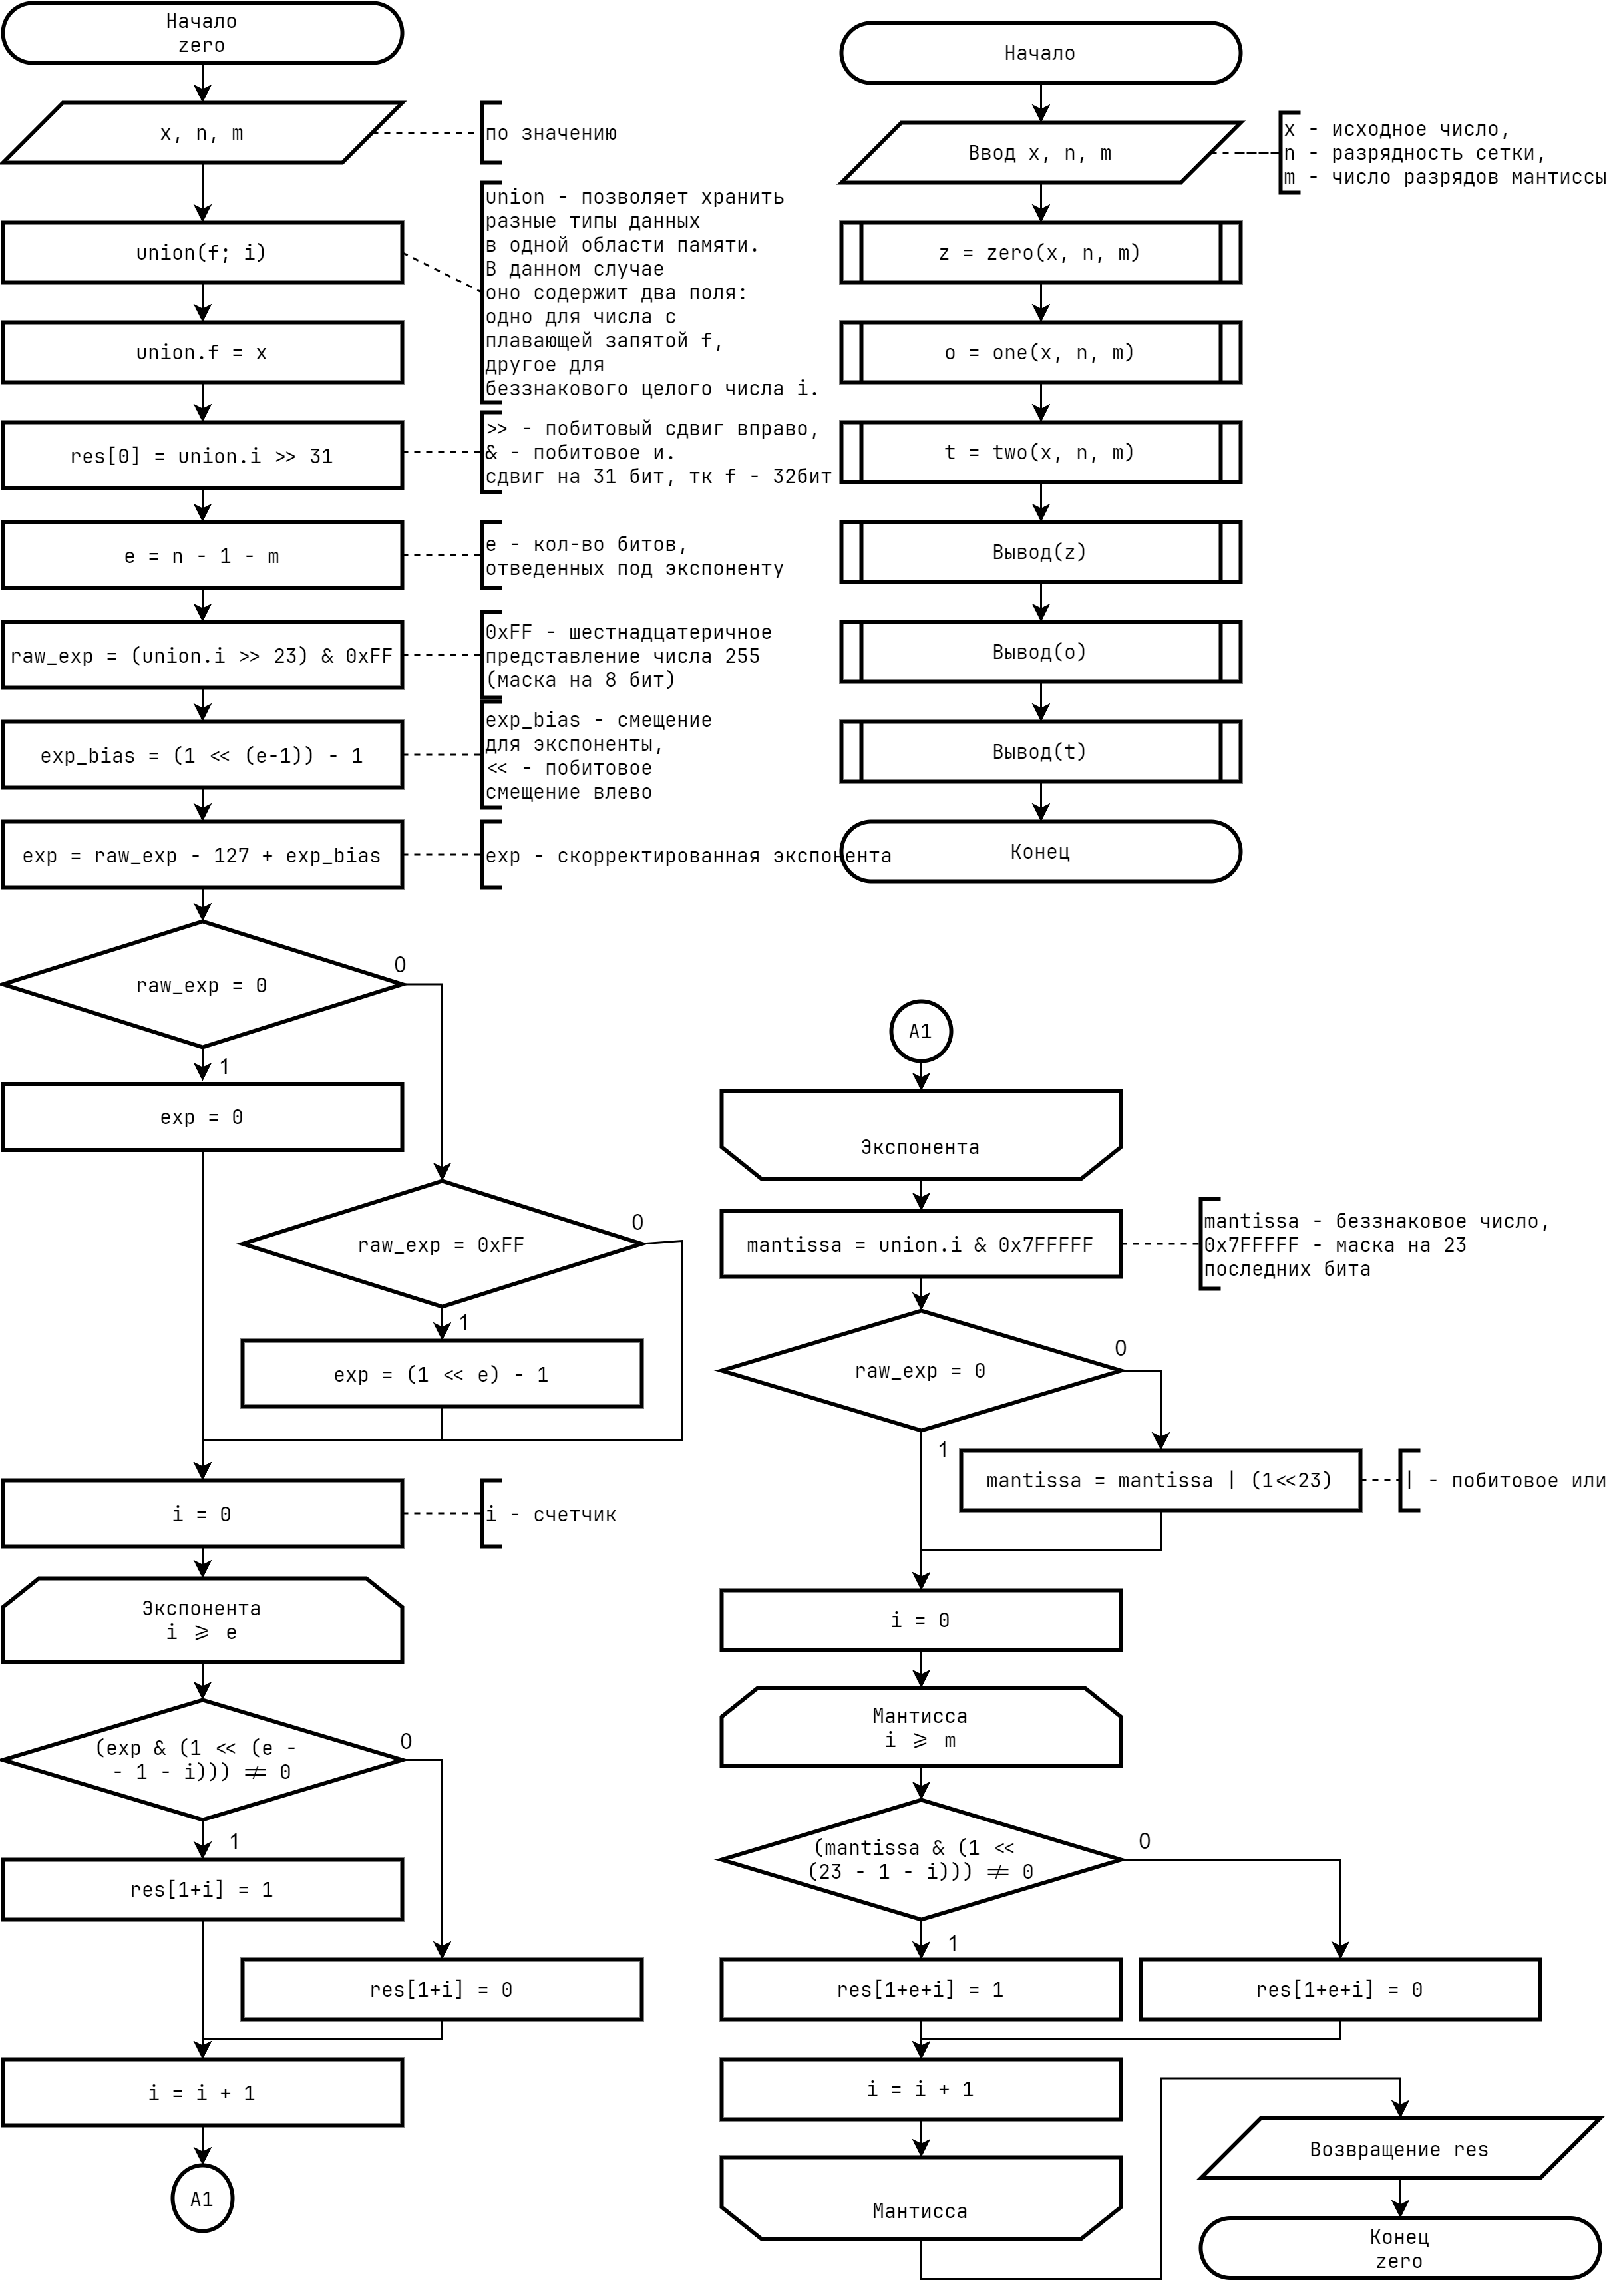
\includegraphics[height=0.75\textheight]{pics/5_flowchart_p1.png}
	\caption*{Рисунок 1.1 - Схема алгоритма программы.}
\end{figure}

\begin{figure}[h!]
	\centering
    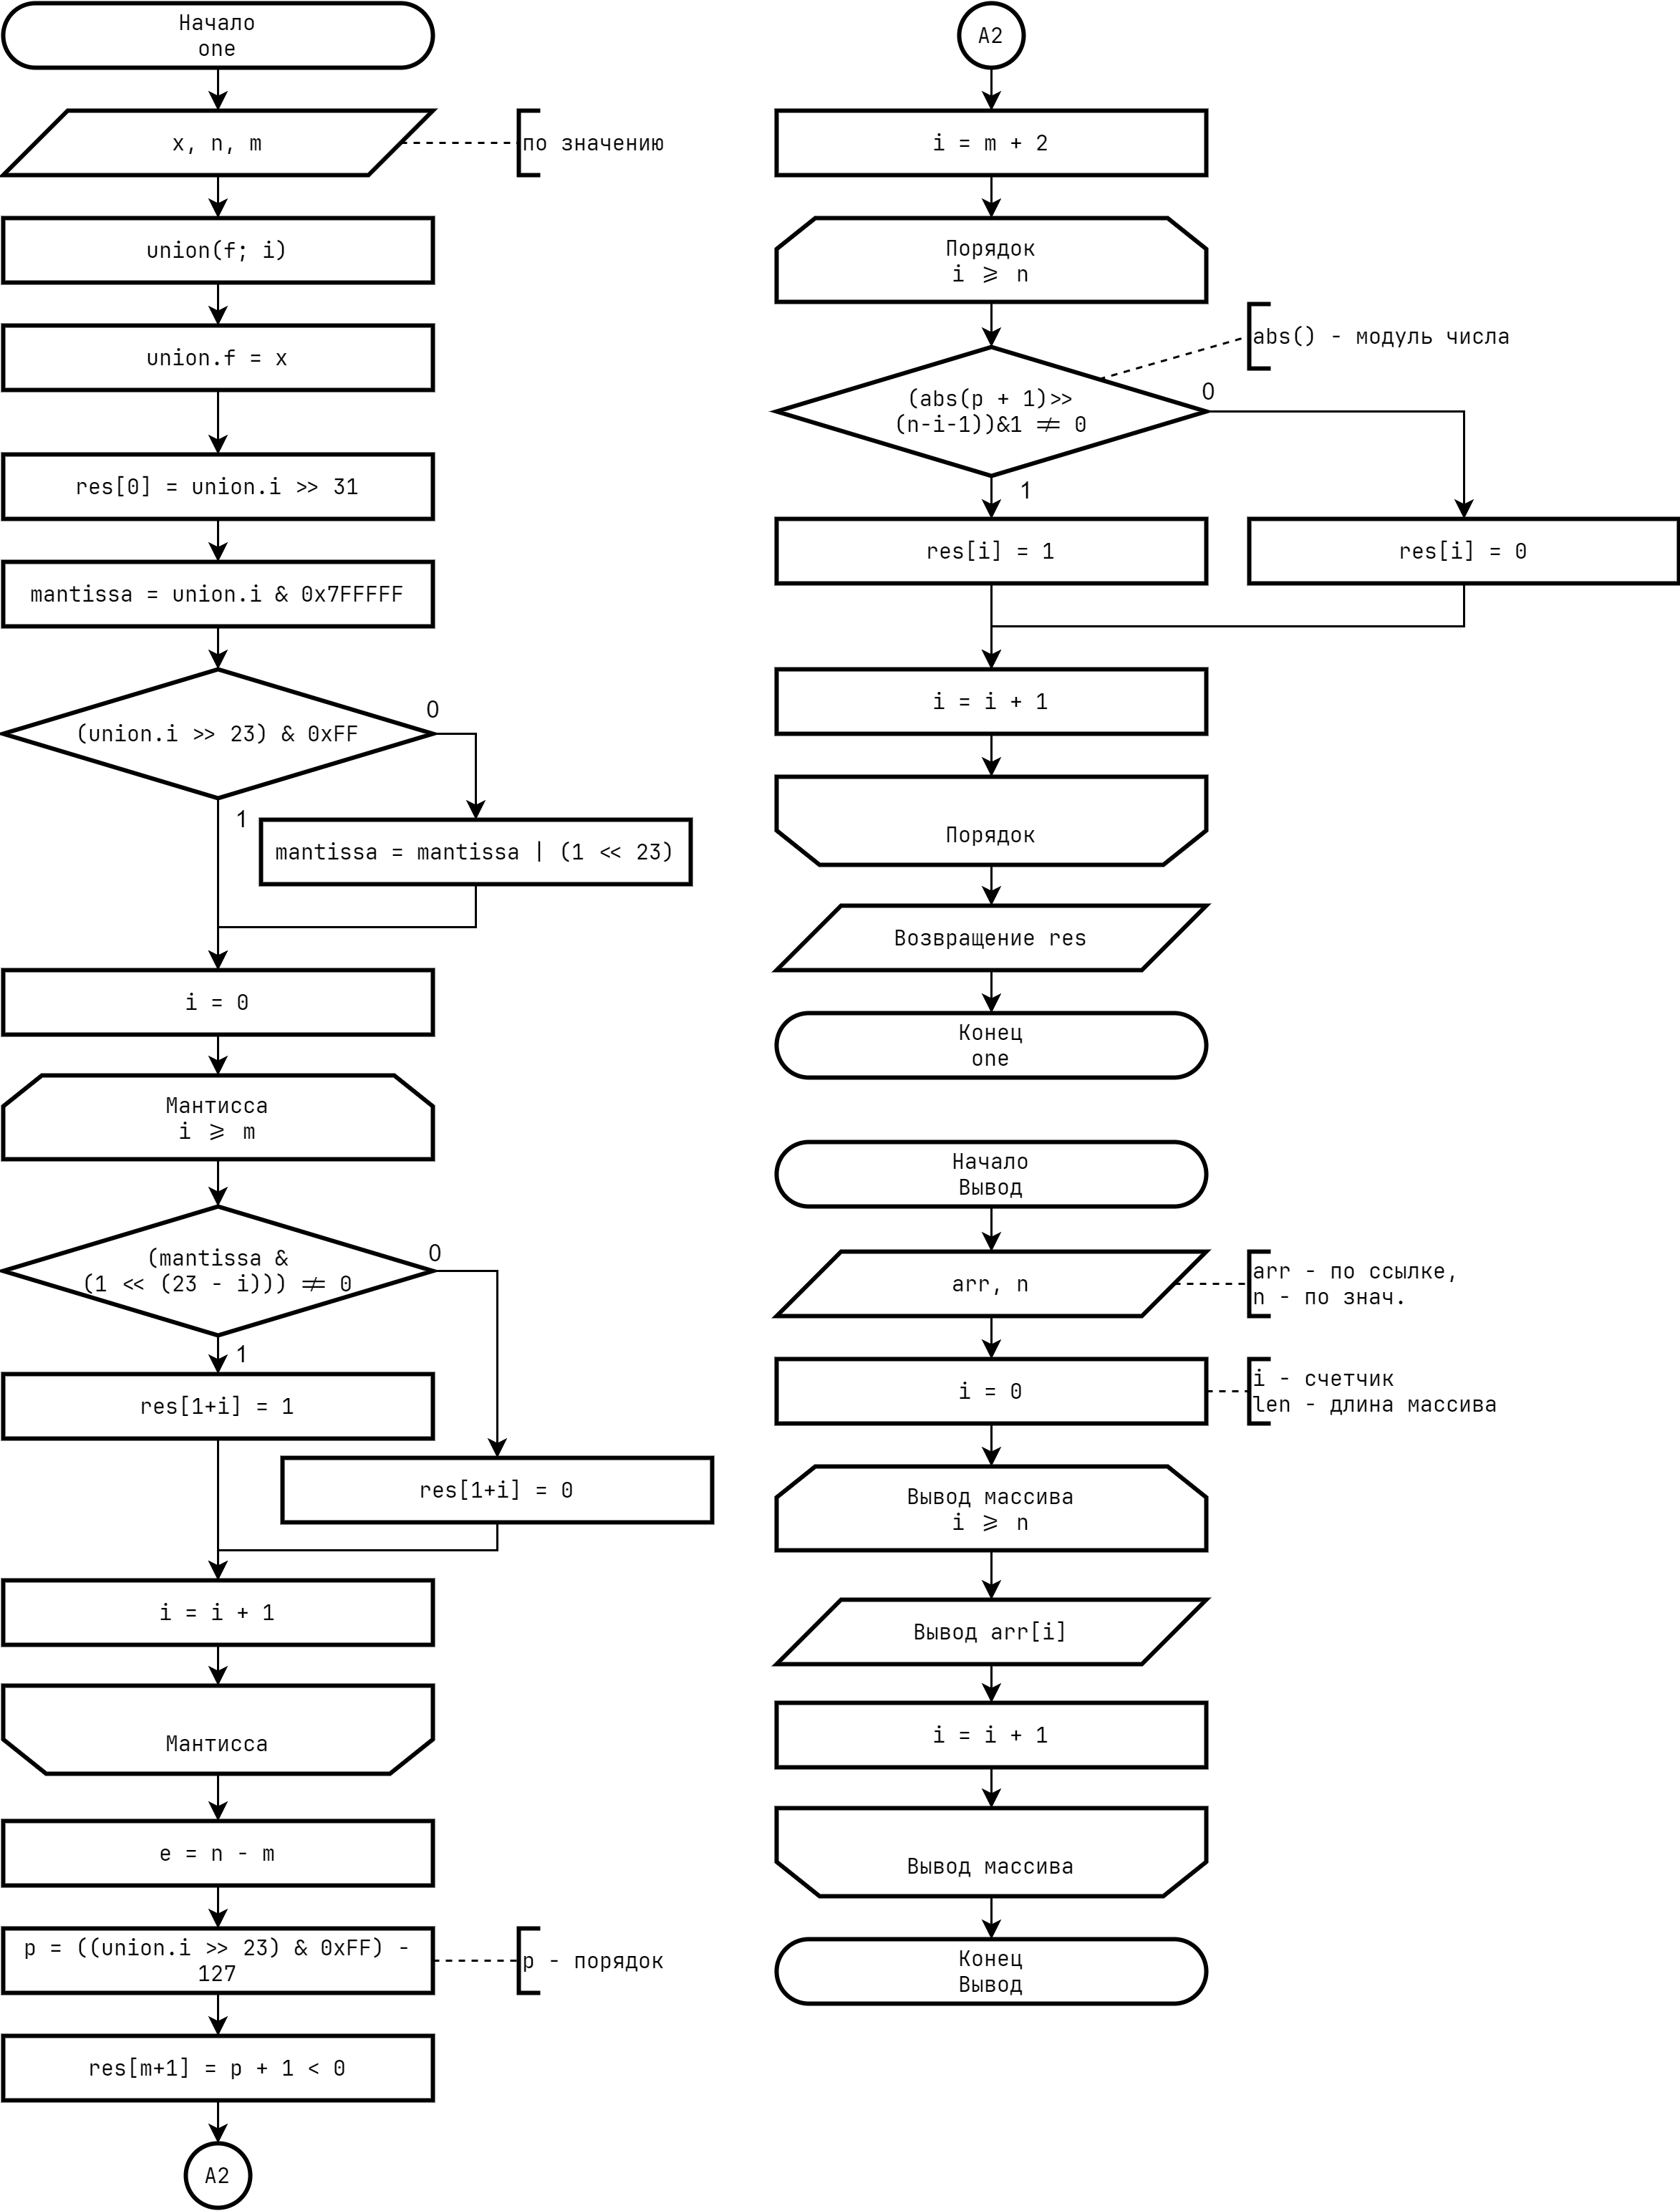
\includegraphics[height=0.9\textheight]{pics/5_flowchart_p2.png}
	\caption*{Рисунок 1.2 - Схема алгоритма программы.}
\end{figure}

\begin{figure}[h!]
	\centering
    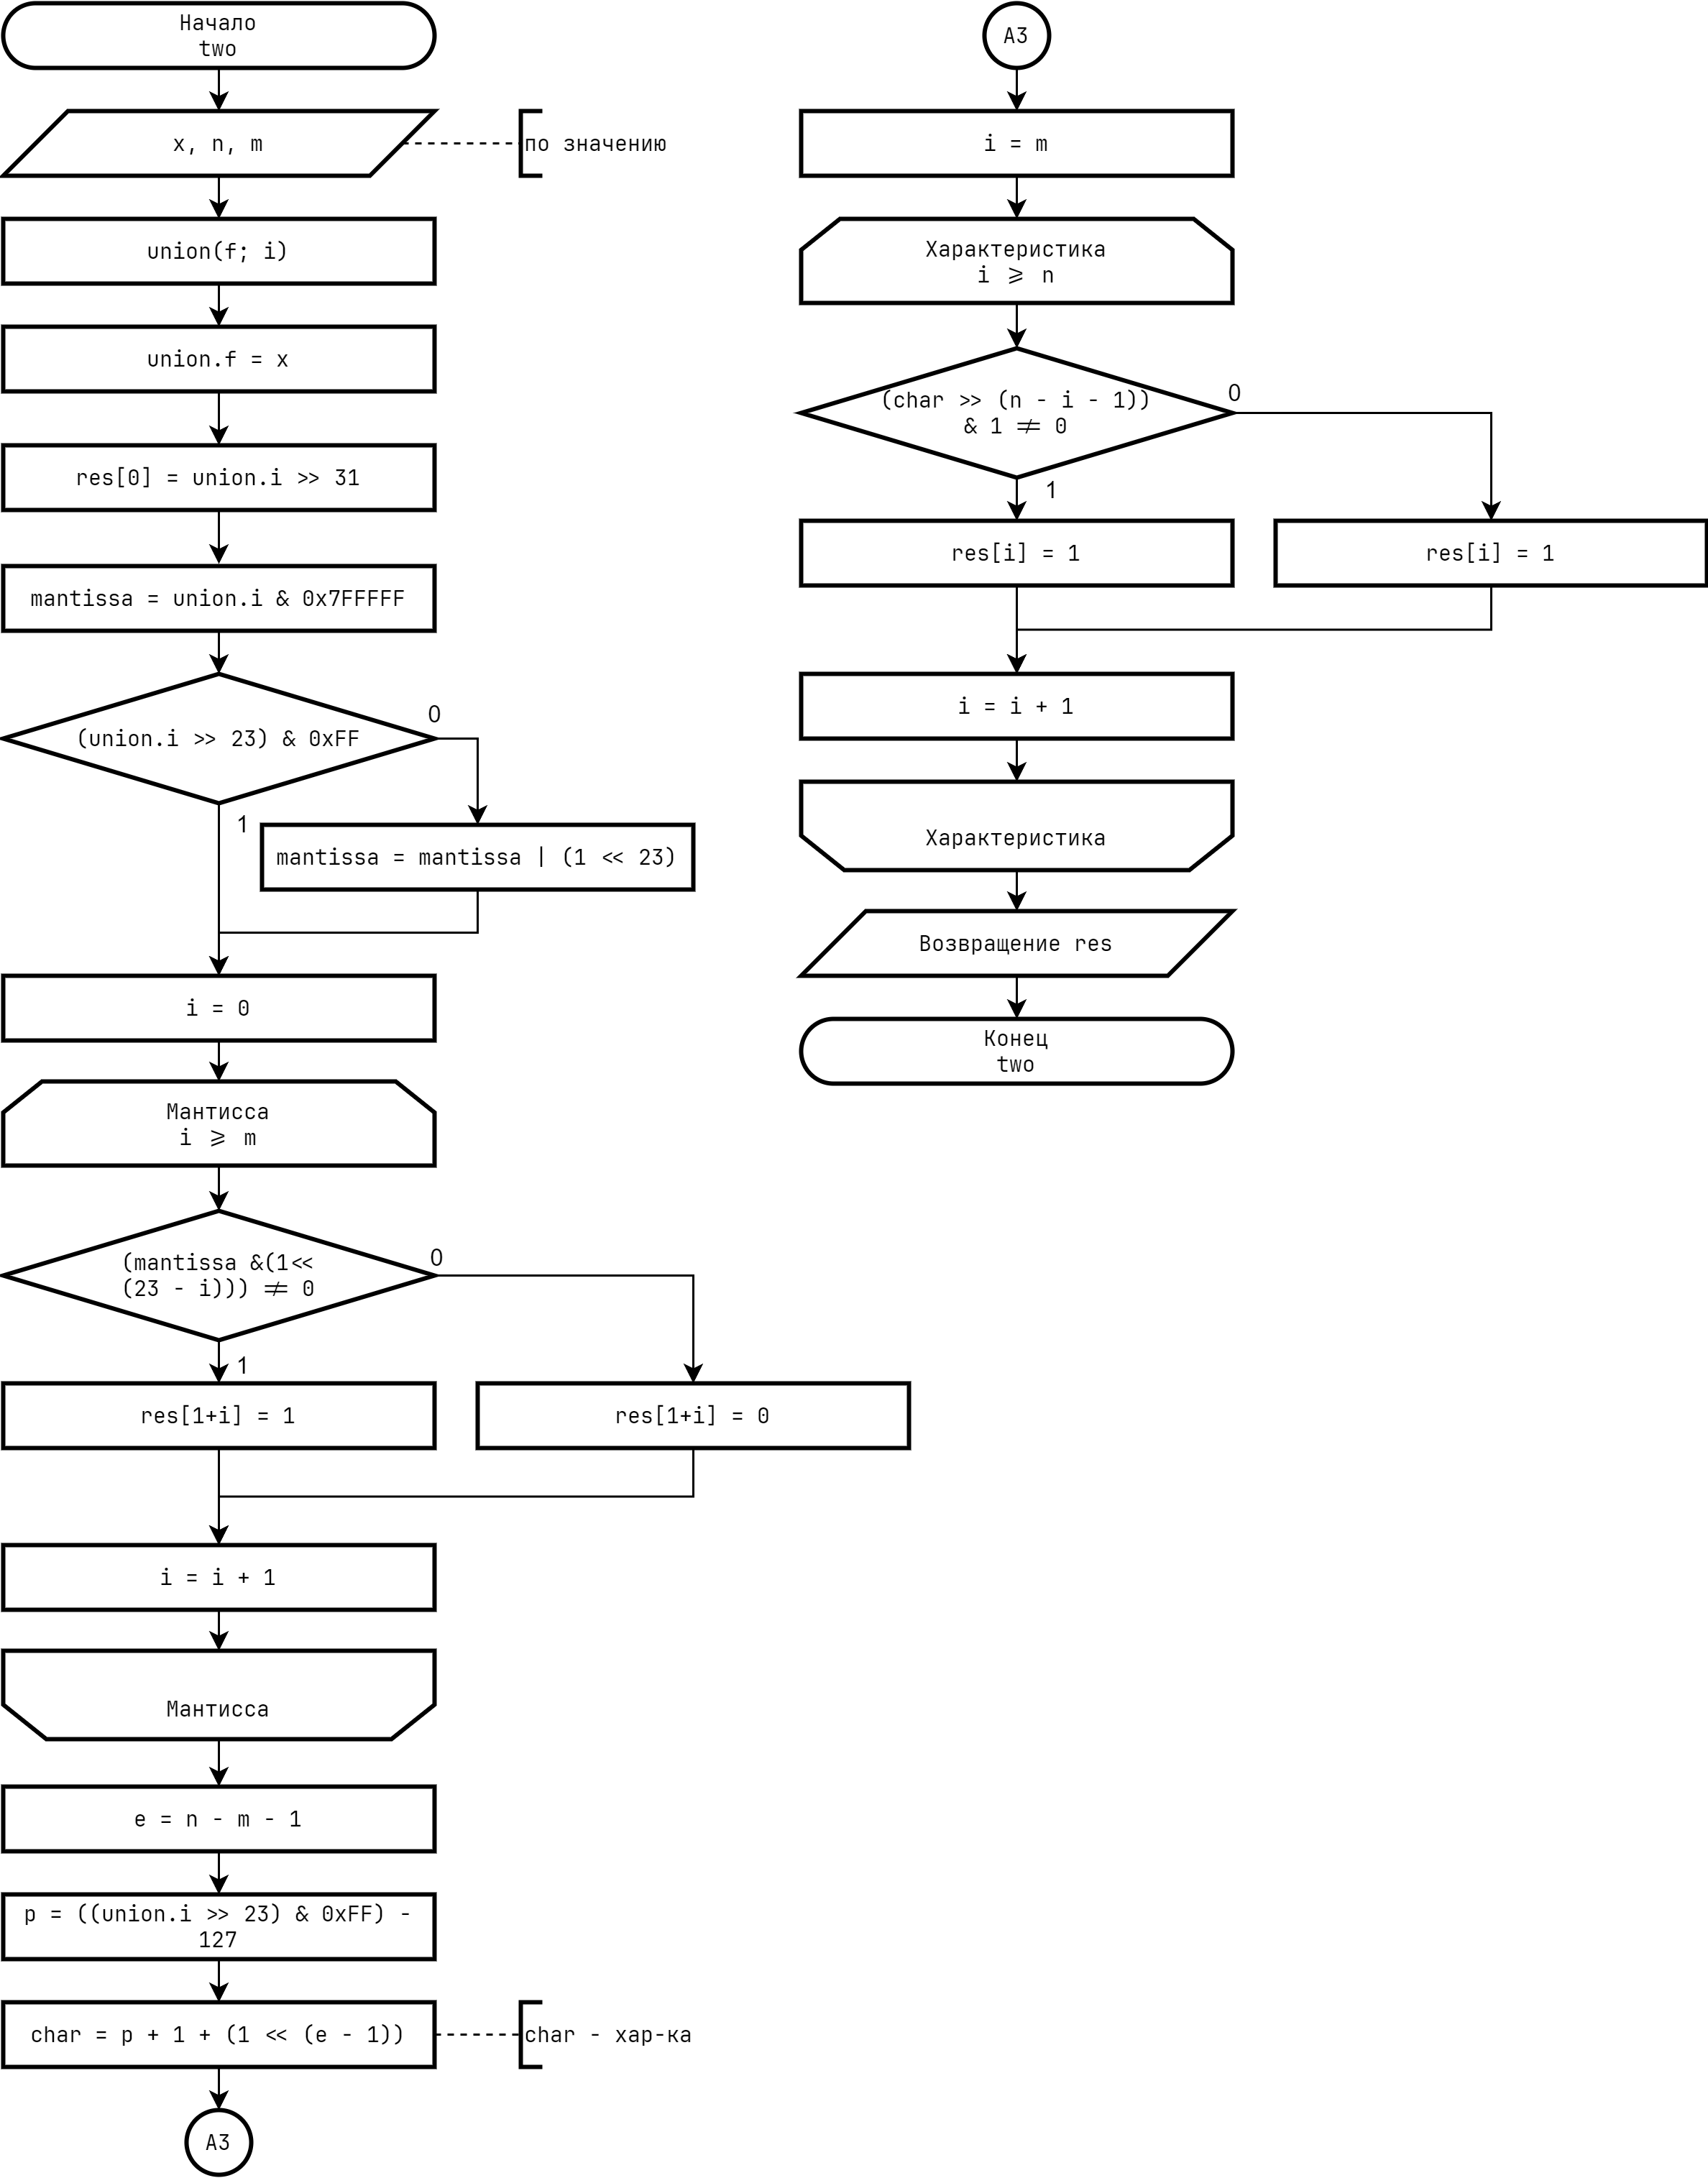
\includegraphics[height=0.9\textheight]{pics/5_flowchart_p3.png}
	\caption*{Рисунок 1.3 - Схема алгоритма программы.}
\end{figure}

\newpage
\section*{Вывод}
В результате работы были разработаны программы для преобразования
вещественных чисел в форматы с плавающей точкой по стандарту. Программы
корректно обрабатывают входные данные и реализуют различные форматы
представления. Тестирование подтвердило их соответствие требованиям.\\

\section*{Приложеие А1}
\VerbatimInput[fontsize=\small]{code/main.c}


\end{document}